\let\negmedspace\undefined
\let\negthickspace\undefined
\documentclass[journal]{IEEEtran}
\usepackage[a5paper, margin=10mm, onecolumn]{geometry}
%\usepackage{lmodern} % Ensure lmodern is loaded for pdflatex
\usepackage{tfrupee} % Include tfrupee package

\setlength{\headheight}{1cm} % Set the height of the header box
\setlength{\headsep}{0mm}     % Set the distance between the header box and the top of the text

\usepackage{xparse}
\usepackage{gvv-book}
\usepackage{gvv}
\usepackage{cite}
\usepackage{amsmath,amssymb,amsfonts,amsthm}
\usepackage{algorithmic}
\usepackage{graphicx}
\usepackage{textcomp}
\usepackage{xcolor}
\usepackage{txfonts}
\usepackage{listings}
\usepackage{enumitem}
\usepackage{mathtools}
\usepackage{gensymb}
\usepackage{comment}
\usepackage[breaklinks=true]{hyperref}
\usepackage{tkz-euclide} 
\usepackage{listings}
\usepackage{gvv}                                        
\def\inputGnumericTable{}                                 
\usepackage[latin1]{inputenc}                                
\usepackage{color}                                            
\usepackage{array}                                            
\usepackage{longtable}                                       
\usepackage{calc}                                             
\usepackage{multirow}                                         
\usepackage{hhline}                                           
\usepackage{ifthen}                                           
\usepackage{lscape}
\begin{document}

\bibliographystyle{IEEEtran}
\vspace{3cm}

\title{9-9.2-41}
\author{EE24BTECH11022 - Eshan Sharma}
% \maketitle
% \newpage
% \bigskip
{\let\newpage\relax\maketitle}

\renewcommand{\thefigure}{\theenumi}
\renewcommand{\thetable}{\theenumi}
\setlength{\intextsep}{10pt} % Space between text and floats


\numberwithin{equation}{enumi}
\numberwithin{figure}{enumi}
\renewcommand{\thetable}{\theenumi}

\textbf{Question}:\\
Area of the region in the first quadrant enclosed by the $x-axis$, the line $y = x$ and the circle $x^{2} + y^{2} = 32$ is
\\
\begin{table}[h!]    
  \centering
  \begin{tabular}[12pt]{ |c|c|c|}
    \hline
    \textbf{Symbol} & \textbf{Value} & \textbf{Description} \\
    \hline
    \textbf{S} & $3cm$ & length of side of square\\
    \hline
    \end{tabular}

  \caption{Variables Used}
  \label{tab0}
\end{table}
\solution\\
The given circle $\vec{C}$ can be expressed as
\begin{align}
	v = \myvec{1&0\\0&1}, u = 0, f = -32
\end{align}
The given line $\vec{L}$ is
\begin{align}
	h = \myvec{1\\-1}
\end{align}
\begin{align}
	\vec{A} = \myvec{4\\4} \text{ and } \vec{B} = \myvec{4\sqrt{2}\\0}
\end{align}
\begin{align}
	\int_{0}^{4} x \, dx + \int_{4}^{4\sqrt{2}} \sqrt{32-x^{2}} \, dx = 4\pi \text{ square units }
\end{align}

\begin{figure}[ht]
    \centering
    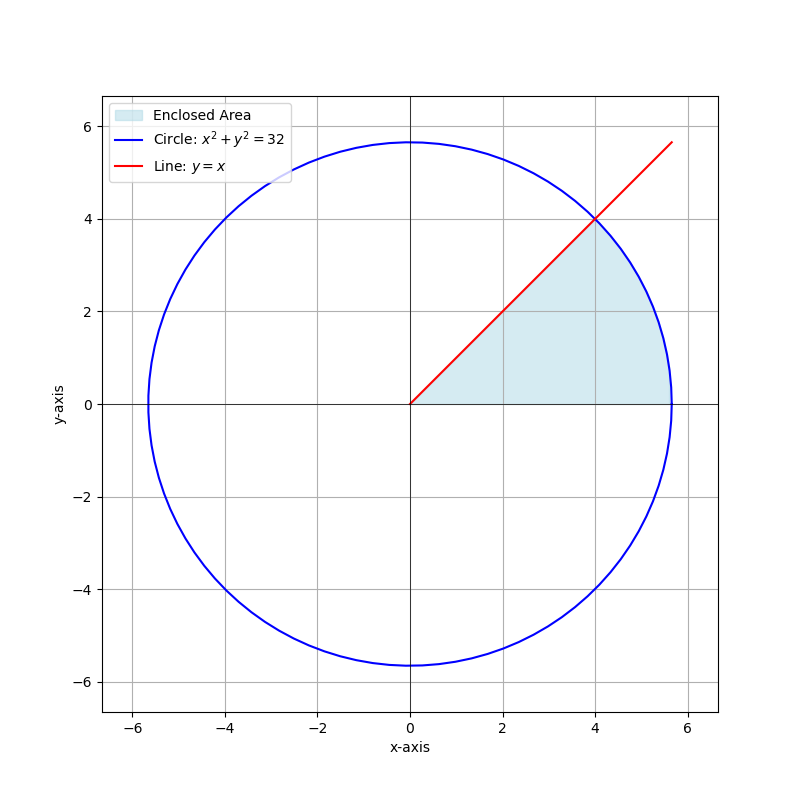
\includegraphics[width=\linewidth]{figs/9-9.2-41.png}
    \caption{Area enclosed in the first quadrant}
\end{figure}
  
\end{document}
